\documentclass[10pt,pdf,hyperref={unicode}, aspectratio=169]{beamer}
% далее идёт преамбула
\usepackage{multirow}
\usepackage{amsmath,amsthm,amssymb}
\usepackage{mathtext}
\usepackage[T1,T2A]{fontenc}
\usepackage[utf8]{inputenc}
\usepackage[english,russian]{babel}
\usepackage[labelfont=bf]{caption}
\usepackage{subcaption}
\usepackage{graphicx}
\usepackage{media9}
\usepackage{multimedia}

\usetheme{Singapore}
\usecolortheme{default}

%\usetheme{Boadilla}
% \usecolortheme{dove}
\usepackage{amsfonts} 
% or 
\usepackage{amssymb}
%ссылки
\usepackage{xcolor}
\usepackage{hyperref}

\definecolor{linkcolor}{HTML}{799B03} % цвет ссылок
\definecolor{urlcolor}{HTML}{799B03} % цвет гиперссылок
 
\hypersetup{pdfstartview=FitH,  linkcolor=blue,urlcolor=blue, colorlinks=true}
%add
\newcommand*{\be}{\begin{equation}}

\newcommand*{\ee}{\end{equation}}

\newcommand*{\ba}{\begin{aligned}}
	\newcommand*{\ea}{\end{aligned}}
\newcommand*{\wt}{\widetilde}
\newcommand{\R}{\mathbb{R}}
\newcommand{\N}{\mathbb{N}}
\newcommand{\Z}{\mathbb{Z}}


\title{\emph{He-Ne laser}}
\subtitle{\underline{laser generation}}
\date{13.03.2021}
\author{Gureva Sonia, Eskoskin Daniil}
\begin{document}

\begin{frame}
\maketitle
\begin{center}

\end{center}
\end{frame}


\begin{frame}{Application.}
	
\begin{columns}
\begin{column}{0.4\linewidth}
\begin{itemize}
	\item \textbf{Cryptography. Chaotic cryptography. Encrypted message transmitting.}\\
	2 synchronised systems (the same parameters) $\to $ synchronised co-evolution $I_1(t) \approx I_2(t) $.
\end{itemize}
\end{column}		
\begin{column}{0.4\linewidth}
\begin{figure}
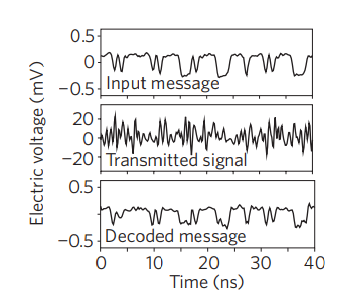
\includegraphics[width=\linewidth]{Encryption.png}
\end{figure}
\end{column}			
%	\includegraphics[scale=0.3]{Hene-1.png}\qquad
\end{columns}
\begin{figure}
	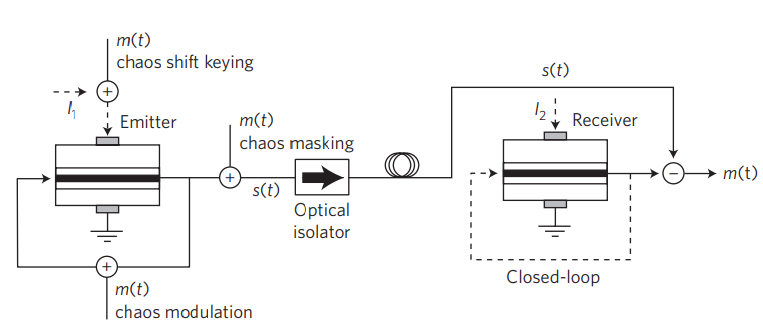
\includegraphics[width=0.4\linewidth]{Encryption_sheme.png}
\end{figure}
\end{frame}


\begin{frame}
\begin{columns}
\begin{column}{0.5\linewidth}		
\begin{itemize}
\item \textbf{Random number generation.}	\\
Random bits produced at a much higher rate than other physical sources of entropy including quantum RNG.	
\item \textbf{Chaos computing.} \\
It is possible to create "NOR" gate\\
"NOR" $\to$ "AND" , "OR", "XOR", "NOT", ... $\to$ computer \\
$\ast$ double-scrolled chaotic attractor and threshold function. 
\end{itemize}
\end{column}
\begin{column}{0.5\linewidth}
	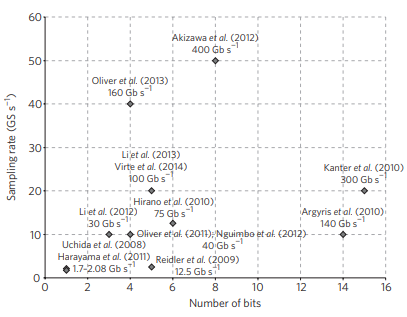
\includegraphics[width=\linewidth]{ChaosRNG.png}
\end{column}
\end{columns}
\end{frame}


\end{document}